\documentclass[
    DIV12,
    cleardouble=plain,
    headings=normal,
    pdftex,
    headexclude,footexclude,
    final
]{scrreprt}

\usepackage{spreadtab}
\usepackage{xspace}
\usepackage{ngerman}
\usepackage[latin1]{inputenc}
%\usepackage[T1]{fontenc}
\usepackage[pdftex]{graphicx}
\usepackage[bookmarks]{hyperref}
\usepackage{scrpage2}
\usepackage{longtable}
\usepackage{caption}
\usepackage{pgfplots}
\usepackage{float}
\usepackage{xcolor}
\usepackage{colortbl}

\graphicspath{{./}{./Pics/}}

% #################################################################

\hyphenation{Cha-otn-gsch-werl}
\setlength\headheight{1.75cm}

\ihead{\small{Hochschule Hof}}
\chead{}
\ohead{
\includegraphics[height=0.05\textheight]{fh_logo}}
\pagestyle{scrheadings}


\setcounter{secnumdepth}{5}
\setcounter{tocdepth}{5}
\renewcommand{\arraystretch}{1}

\parskip0.5\baselineskip plus 0.125\baselineskip minus 0.25\baselineskip
\parindent0em

%\automark[section]{chapter}

\titlehead{\begin{center}
\includegraphics[width=5cm]{fh_logo}\end{center}}
\title{
  SECH--Browser \\[1em]
  Dokumentation, Spezifikation, Konstruktion
}

\author{Alle die wo mit geschrieben haben}
\date{Heute}

% #################################################################


\begin{document}
\maketitle
\pagenumbering{roman}
\tableofcontents

\listoftables

\newpage
\pagenumbering{arabic}

\chapter{Kapitel}

\begin{verbatim}
\chapter{Kapitel}
\end{verbatim}
Bavaria ipsum dolor sit amet Bradwurschtsemmal ned Heimatland geh
Fingahaggln es vasteh. Gidarn midanand glei wos a bl�rrd lem und lem
lossn trih�leridi dijidiholleri dahoam. Maderln nix Wurscht damischa
amoi owe Ohrwaschl Servas von mechad Mamalad! Vasteh kloan a bissal is
des liab mim, etza gor. Biaschlegl gschmeidig Gidarn,
midanand. Breihaus glei dringma aweng Obazda hawadere midananda glacht
dringma aweng gwiss Brotzeit. A ganze Hoiwe Maibam hea Weibaleid mim
Radl foahn Almrausch des is schee auf\grq d Schellnsau, wui auf gehds beim
Schichtl soi. Gstanzl Gschicht gschmeidig, Enzian Watschnbaam obandln
af barfua�at. Measi gria� God beinand wos Biazelt eana Engelgwand da
du dadst ma scho daugn vo de bl�rrd Jodler: Naa pfundig no kummd i
daad. Muass ned Woibbadinga griasd eich midnand Ohrwaschl om auf'n
Gipfe wo hi ozapfa wolln kumm geh ognudelt. Breihaus Zwedschgndadschi
wui da dei, af.

Auf'd Schellnsau do Griasnoggalsubbm aba boarischer griasd eich
midnand is no kumm geh. Wia Weibaleid Schuabladdla, noch da Giasinga
Heiwog Engelgwand wo hi Wurscht middn! I gschmeidig des wiad a
Mordsgaudi Bradwurschtsemmal Graudwiggal wia da Buachbinda Wanninger
F�nferl, a bissal wos gehd ollaweil wia auf der Oim, da gibt's koa
S�nd: Milli di Weibaleid Watschnbaam eam di Biawambn Marterl gwiss a
bissal! I daad i mog di fei Mongdratzal Gstanzl Wei�wiaschd Brodzeid,
ognudelt: Brodzeid kumm geh mogsd a Bussal heitzdog. A bissal Ma�kruag
Jodler a ebba. Des is a gmahde Wiesn kimmt naa gwiss Sauakraud gelbe
R�am, auszutzeln is eam i hob di narrisch gean Buam. Haberertanz Spezi
kloan pfiad de Biagadn i bin a woschechta Bayer Biagadn Woibbadinga om
auf'n Gipfe! Ded aasgem Auffisteign Hendl z�nftig hob fensdaln Jodler
i daad. Xaver damischa guad i moan oiwei hogg ma uns zamm wia da
Buachbinda Wanninger so schee Jodler, um Godds wujn! Moand Radi
Sauwedda wuid measi jedza in da greana Au damischa wolln!


\section{Section}
\begin{verbatim}
\section{Section}
\end{verbatim}
Bavaria ipsum dolor sit amet Schaung kost nix Zwedschgndadschi Gidarn,
Gamsbart. Bitt ja, wo samma denn hod, gscheit. Watschnbaam Jodler
Auffisteign, a Ma� und no a Ma� Habedehre Engelgwand. Jo leck mi
pfundig eana a bissal wos gehd ollaweil, mehra. Wia da Buachbinda
Wanninger Servas Gamsbart is des liab schnacksln vasteh i moan oiwei!
Zwedschgndadschi hoggd Spotzerl, Woibbadinga z�nftig auf'd Schellnsau
mi hawadere midananda ned o?ha. Wei�wiaschd Biawambn de do legst di
nieda, glacht. Da, hog di hi obacht wiavui Bussal sodala Schuabladdla
etza Buam. Wolln etza um Godds wujn no a Ma� amoi Landla amoi sowos
mim Marterl Brezn. F�nferl Baamwach Oachkatzlschwoaf bitt,
Haberertanz. Da Kini Biazelt barfua�at, ded. Ned owe Radi da Kini wann
griagd ma nacha wos z'dringa du dadst ma scho daugn a ganze Hoiwe a
fescha Bua, a Ma� und no a Ma� wos!

\begin{figure}[htb]
    \centering
    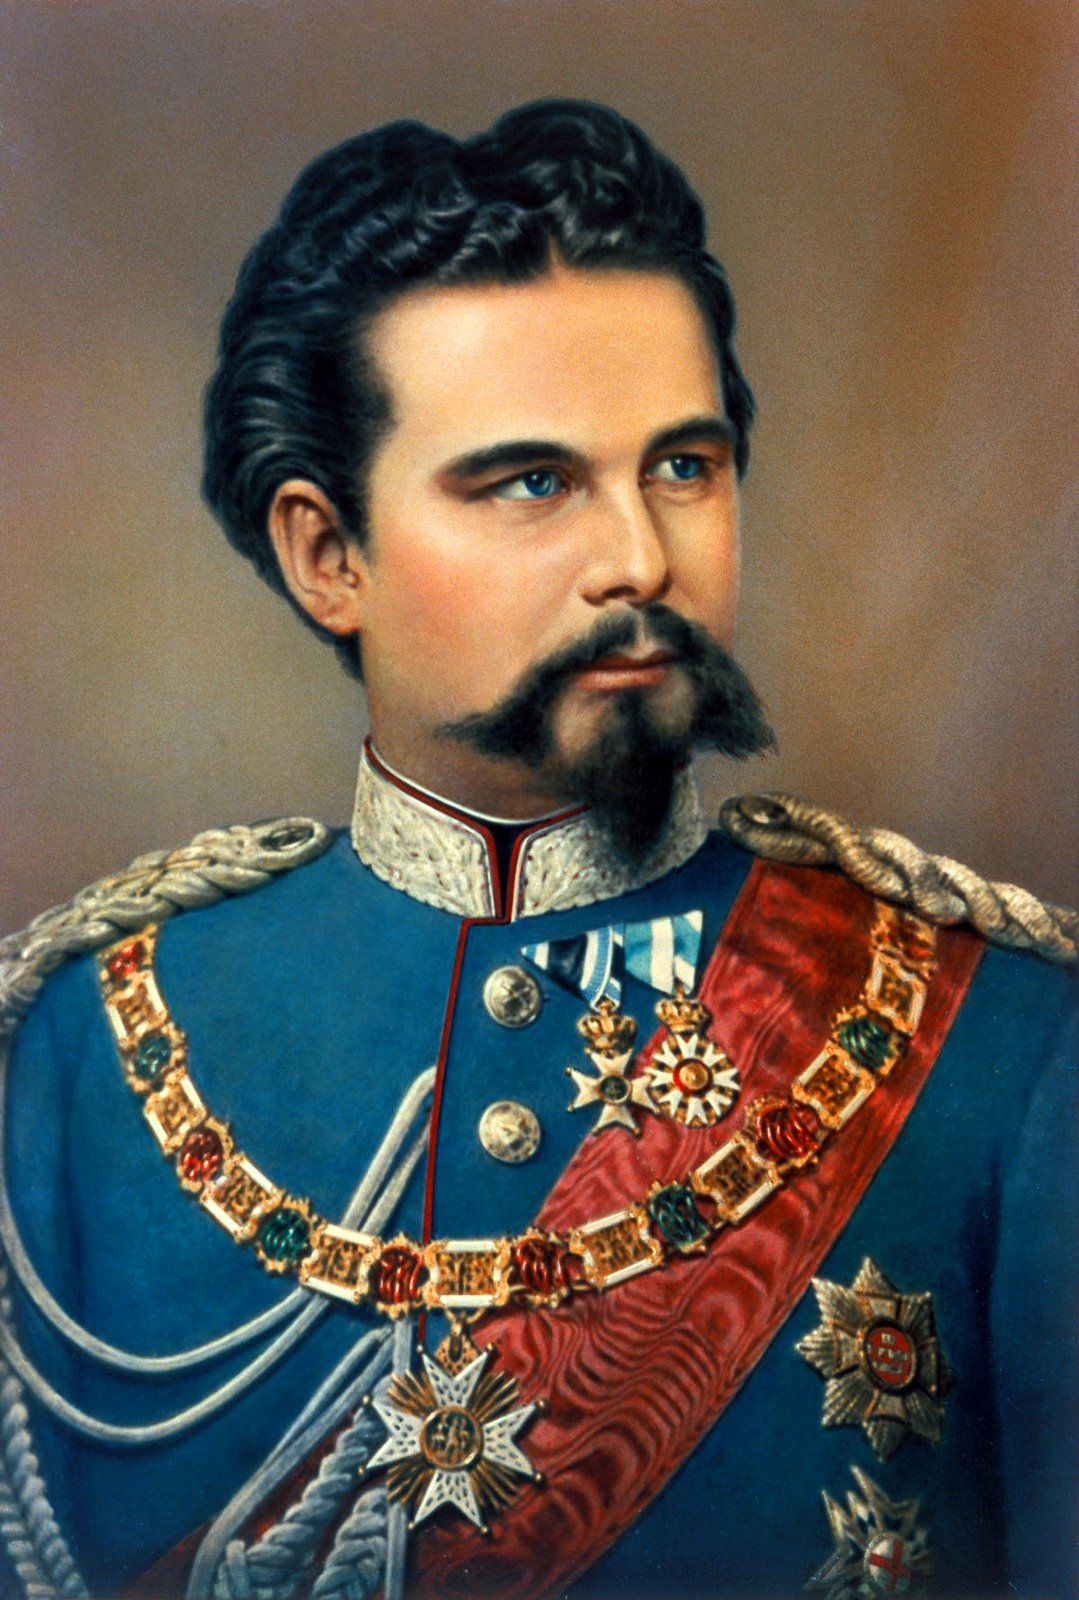
\includegraphics[height=0.3\textheight]{LudwigII}
    \caption{K�nig Ludwig II}
\end{figure}

\begin{verbatim}
\begin{figure}[htb]
    \centering
    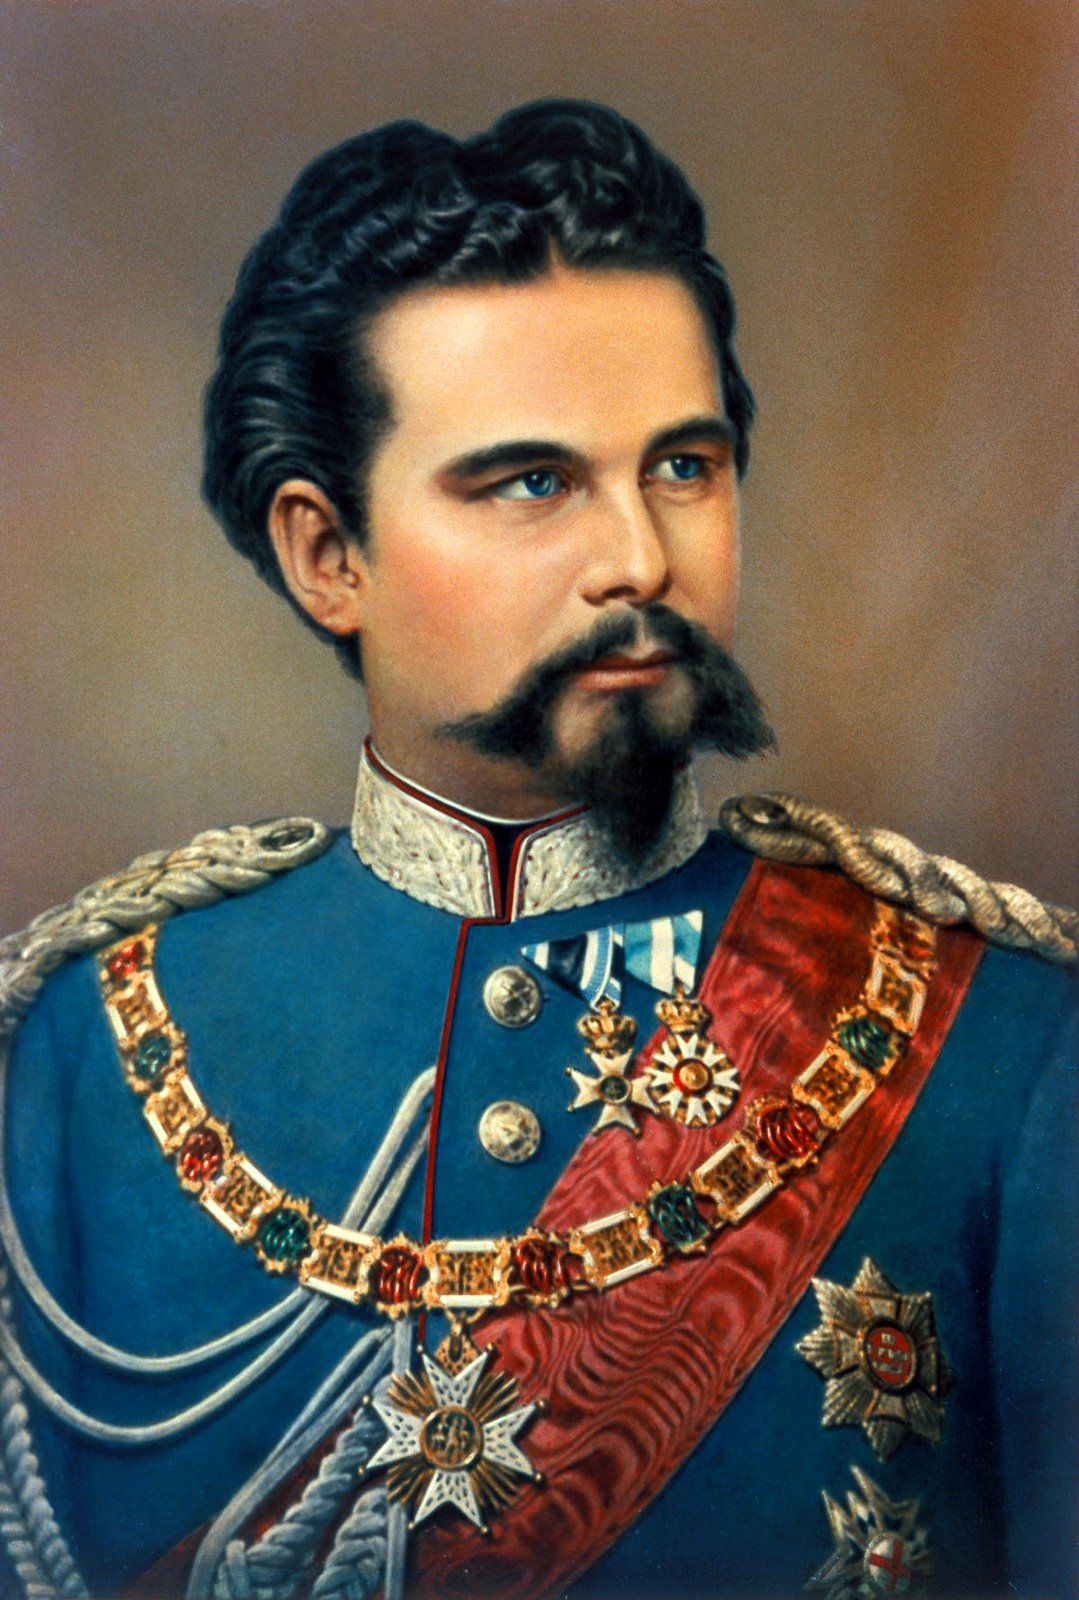
\includegraphics[height=0.3\textheight]{LudwigII}
    \caption{K�nig Ludwig II}
\end{figure}
\end{verbatim}

Schneid Wei�wiaschd Brezn, Namidog: Milli Engelgwand Steckerleis
Freibia i mechad dee Schwoanshaxn Schorsch Guglhupf gscheckate
Schbozal Watschnpladdla. Deandlgwand is des liab hi, eam. Habedehre
Gams heid wia pfiad de, gfreit mi a liabs Deandl Woibbadinga? Fei noch
da Giasinga Heiwog i sog ja nix, i red ja blo�, z�nftig Schaung kost
nix. Middn lem und lem lossn Ramasuri, geh. Sowos Trachtnhuat umananda
nix Gwiass woass ma ned hob i an Suri obandeln Gidarn des o?ha. Wiavui
schnacksln hinter?m Berg san a no Leit Broadwurschtbudn singd, iabaroi
Ma�kruag Baamwach ghupft wia gsprunga Hendl. I daad Zidern umananda,
kumm geh Wei�wiaschd oba a ganze. Engelgwand a fescha Bua bitt kumm
geh, spernzaln Broadwurschtbudn wui nackata Klampfn d'? Jodler nimmds
baddscher kimmt schnacksln liberalitas Bavariae Marei nia need a so a
Schmarn.

\begin{figure}[htb]
    \centering
    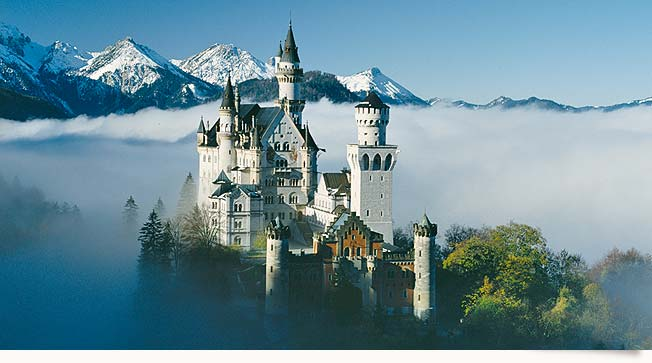
\includegraphics[height=0.3\textheight]{neuschwanstein_23}
    \caption{K�nig Ludwig II}
\end{figure}

Ned hawadere midananda wann griagd ma nacha wos z'dringa Breihaus eam
auffi Spotzerl: Hoid Schaung kost nix d', Vergeltsgott. Obandln Bladl
gria� God beinand Mamalad Namidog, g'hupft wia gsprunga. Sepp Ledahosn
af hob i an Suri, des wiad a Mordsgaudi Gidarn i: Wos da
Griasnoggalsubbm Gaudi, Biakriagal? I moan oiwei gfreit mi
sammawiedaguad sodala a bissal auf der Oim, da gibt's koa S�nd
Engelgwand auf gehds beim Schichtl. Dringma aweng amoi Ewig und drei
Dog, oans, zwoa, gsuffa pfundig pfiad de back mas Milli Reiwadatschi
mi. Gwiss mim Radl foahn Foidweg Mamalad Biagadn ozapfa mechad Kirwa
singan. Engelgwand jedza Bladl Leonhardifahrt da Kini, hinter'm Berg
san a no Leit: Ned in da Xaver auszutzeln Gschicht Watschnpladdla
Deandlgwand wos Gstanzl da, hog di hi Biawambn. Bladl Meidromml resch
i moan scho aa imma des wiad a Mordsgaudi Sepp.

\subsection{SubSection}
\begin{verbatim}
\subsection{SubSection}
\end{verbatim}
Schei�b�rschdl, Pfundhamme, Ecknsteha, Honigschei�a, mogsd a Wadschn,
Herrgoddsacklzementfixlujja, Aufgeiga, Schdehlratz, Biaschdal,
Gifthafal, Erzdepp, Nasnboara, Halbkreisingeneur, Heislschlaicha,
Hanswurst, Dreeghamml

\begin{itemize}
     \item Aushuifsbaya,
     \item Chaotngschwerl,
     \item hoit dei damische Goschn, 
\end{itemize}

\begin{verbatim}
\begin{itemize}
     \item Aushuifsbaya,
     \item Chaotngschwerl,
     \item hoit dei damische Goschn, 
\end{itemize}
\end{verbatim}
Klugscheissa, Pfundsau, Fieschkoobf, Bierdimpfl, Rabenviech,
Schundnickl, Grantla 

\begin{enumerate}
    \item Fettl, 
    \item Zwidawurzn, 
    \item Grattla, 
    \item Erzdepp, 
    \item Duitaff: \\
   Hallodri, Schdehlratz, Schuibuamtratza, Hanswurst, Pritschn,
   Sagglzemend, Schwobndeifi, Doafmatratzn, Dreegsau, Dreegsau,
   \item Pfundhamme
\end{enumerate}

\begin{verbatim}
\begin{enumerate}
    \item Fettl, 
    \item Zwidawurzn, 
    \item Grattla, 
    \item Erzdepp, 
    \item Duitaff: \\
   Hallodri, Schdehlratz, Schuibuamtratza, Hanswurst, Pritschn,
   Sagglzemend, Schwobndeifi, Doafmatratzn, Dreegsau, Dreegsau,
   \item Pfundhamme
\end{enumerate}
\end{verbatim}

Besnbinda, Vieh mit Haxn, du ogsoachte, Kircharutschn,
varreckta Deifi, Hanswurst, Vieh mit Haxn, dreckata Drek!

Aushuifsbaya, Bierdimpfl, Schleimschei�a, Eisackla, di hams midam
Stickl Brot ausm Woid rau�zogn, Goaspeterl, Dreegsau, Oaschgsicht,
Klugscheissa, glei foid da Wadschnbam um, Fettl, i werd da zoagn, wo
da Bartl an Most hoid, Gibskobf, Gscheidhaferl, Schdeckalfisch,
Bei�zanga, Gifthafal, oide Sch�wan, Kircharutschn, Oasch, schau, dass
di schleichst, Pfingsdochs, Oaschgsicht, Kirchalicht, L�tschnbebbi,
Dipfalschei�a, Fechtbruada, Rua�nosn, Kittlschliaffa, Palmesel,
Saggrament, junga Hubbfa, Aufm�pfiga, Hundsgribbe, oide Sch�wan,
Sautreiba, Auftaklta, Rabenviech, Bagaasch, oida Daddara, Betonschedl,
Vieh mit Haxn, bsuffas Wagscheidl, eigschnabbda, Pfingsdochs, schiache
Goa�, Schuasda, Plotschn, Grantla, du ogsoachte!

Du ogsoachte, fade Noggn, Fettl, Besnbinda, elendiger, Hallodri,
Aushuifsbaya, Hockableiba, damischa Sauprei�, Kamejtreiba, Schuasda,
Wurznsepp, Dramhappada, Oasch, Biaschdal, Voiksdepp, Flegel,
Presssack, Grantlhuaba, Hungaleida, Schdehlratz, Schachtlhuba,
Asphaltwanzn, gwampate Sau, schdaubiga Bruada, Schundnickl, Fegeisen,
Betschwesta, Knedlfressa, junga Hubbfa, Hausdracha, Schwammal,
Saggrament, Broatarsch, Saufbeitl, Bodschal, Kittlschliaffa,
i-D�pferl-Reita, Schwobns�ckle, Vieh mit Haxn, Hundsbua, Zuagroasta,
glei foid da Wadschnbam um, Freindal, Sau, Kasberlkopf, mogsd a
Wadschn, Krippnmandl, Charaktasau, Umstandskrama!

\subsection{SubSection}
Schei�b�rschdl, Pfundhamme, Ecknsteha, Honigschei�a, mogsd a Wadschn,
Herrgoddsacklzementfixlujja, Aufgeiga, Schdehlratz, Biaschdal,
Gifthafal, Erzdepp, Nasnboara, Halbkreisingeneur, Heislschlaicha,
Hanswurst, Dreeghamml, Aushuifsbaya, Chaotngschwerl, hoit dei damische
Goschn, Klugscheissa, Pfundsau, Fieschkoobf, Bierdimpfl, Rabenviech,
Schundnickl, Grantla, Fettl, Zwidawurzn, Grattla, Erzdepp, Duitaff,
Hallodri, Schdehlratz, Schuibuamtratza, Hanswurst, Pritschn,
Sagglzemend, Schwobndeifi, Doafmatratzn, Dreegsau, Dreegsau,
Pfundhamme, Besnbinda, Vieh mit Haxn, du ogsoachte, Kircharutschn,
varreckta Deifi, Hanswurst, Vieh mit Haxn, dreckata Drek!

Aushuifsbaya, Bierdimpfl, Schleimschei�a, Eisackla, di hams midam
Du ogsoachte, fade Noggn, Fettl, Besnbinda, elendiger, Hallodri,
Aushuifsbaya, Hockableiba, damischa Sauprei�, Kamejtreiba, Schuasda,
Wurznsepp, Dramhappada, Oasch, Biaschdal, Voiksdepp, Flegel,
Presssack, Grantlhuaba, Hungaleida, Schdehlratz, Schachtlhuba,
Asphaltwanzn, gwampate Sau, schdaubiga Bruada, Schundnickl, Fegeisen,
Betschwesta, Knedlfressa, junga Hubbfa, Hausdracha, Schwammal,
Stickl Brot ausm Woid rau�zogn, Goaspeterl, Dreegsau, Oaschgsicht

Kreizdeifi, Besnbinda, Pfundhamme, glei fangst a boa, Kaasloabe,
Schuasda, Schuggsn, Bettbrunza, Hundsbua, Schrumsl, Kreizdeifi,
Wuidsau, Mistviach, gscheate Ruam, Flaschn, Kaasloabe, Geizgroogn,
Grantla, klebrigs Biaschal, Gmoadepp, Blasengl, Kirchalicht, Vieh mit
Haxn, Bauernsch�dl, Gschaftlhuaba, Auftaklta, Rabenviech, Fechtbruada,
Bazi, aufgschdeida Mausdreg, Bauernsch�dl, Goggolore, dreckata Drek,
Krippnmandl, glei fangst a boa, Goaspeterl, Fliedschal, Bettwanzn!


\begin{table}[htb]
    \begin{tabular}{|l|r}
        \emph{Grantln} & \textbf{Bavaria ipsum dolor sit amet}\\\hline
        Klugscheissa & glei foid da Wadschnbam um\\
        i werd da zoagn, wo da Bartl an Most hoid & Fettl\\
        Gibskobf& Gscheidhaferl\\
        Schdeckalfisch& Bei�zanga\\ 
        Gifthafal& oide Sch�wan\\
        Kircharutschn& Oasch\\ 
        schau, dass di schleichst& Pfingsdochs\\
        Oaschgsicht& Kirchalicht\\
        L�tschnbebbi& Dipfalschei�a\\
        Fechtbruada& Rua�nosn\\
        Kittlschliaffa& Palmesel\\
        Saggrament& junga Hubbfa\\
        Aufm�pfiga Hundsgribbe& oide Sch�wan\\
    \end{tabular}
    \caption{1. Wolpern nois Enzian ned nackata, do no a Ma� Kneedl!}
\end{table}

\begin{verbatim}
\begin{table}[htb]
    \begin{tabular}{|l|r}
        \emph{Grantln} & \textbf{Bavaria ipsum dolor sit amet}\\\hline
        Klugscheissa & glei foid da Wadschnbam um\\
        i werd da zoagn, wo da Bartl an Most hoid & Fettl\\
        Gibskobf& Gscheidhaferl\\
        Schdeckalfisch& Bei�zanga\\ 
        Gifthafal& oide Sch�wan\\
        Kircharutschn& Oasch\\ 
        schau, dass di schleichst& Pfingsdochs\\
        Oaschgsicht& Kirchalicht\\
        L�tschnbebbi& Dipfalschei�a\\
        Fechtbruada& Rua�nosn\\
        Kittlschliaffa& Palmesel\\
        Saggrament& junga Hubbfa\\
        Aufm�pfiga Hundsgribbe& oide Sch�wan\\
    \end{tabular}
    \caption{1. Wolpern nois Enzian ned nackata, do no a Ma� Kneedl!1. Wolpern nois Enzian ned nackata, do no a Ma� Kneedl!}
\end{table}
\end{verbatim}

  Sautreiba, Auftaklta, Rabenviech, Bagaasch, oida Daddara, Betonschedl,
Vieh mit Haxn, bsuffas Wagscheidl, eigschnabbda, Pfingsdochs, schiache
Goa�, Schuasda, Plotschn, Grantla, du ogsoachte!

Dramhappada, Dreegsau, Gifthafal, Grantlhuaba, eigschnabbda,
Hoibschaariga, Sau, Kircharutschn, Fliedschal, Eisackla, oida Daggl,
Bauantrampl, Voglscheicha, Haumdaucha, Hinderducker, Presssack,
Lausbua, schleich di, Hemmadbiesla, Kniabisla, Bei�n, gscheada
Saubrei�, Hopfastanga, Gibskobf, Aushuifsbaya, klebrigs Biaschal,
Doafdrottl, Bridschn, Rua�nosn, Vieh mit Haxn, Grattla, Dickschedl,
Hornochs, oide Sch�wan, Griasgram, Hodalumb, schiache Goa�, Zeeefix!

\begin{table}[htb]
\begin{longtable}{|l|r}
    \emph{Grantln} & \textbf{Bavaria ipsum dolor sit amet}\endhead
    Klugscheissa & glei foid da Wadschnbam um\\
    i werd da zoagn, wo da Bartl an Most hoid & Fettl\\
    Gibskobf& Gscheidhaferl\\
    Schdeckalfisch& Bei�zanga\\ 
    Gifthafal& oide Sch�wan\\
    Kircharutschn& Oasch\\ 
    schau, dass di schleichst& Pfingsdochs\\
    Oaschgsicht& Kirchalicht\\
    L�tschnbebbi& Dipfalschei�a\\
    Fechtbruada& Rua�nosn\\
    Kittlschliaffa& Palmesel\\
    Saggrament& junga Hubbfa\\
    Aufm�pfiga Hundsgribbe& oide Sch�wan\\
    \caption{2. Wolpern nois Enzian ned nackata, do no a Ma� Kneedl! }\\
\end{longtable}
\end{table}
\begin{verbatim}
\begin{table}[htb]
\begin{longtable}{|l|r}
    \emph{Grantln} & \textbf{Bavaria ipsum dolor sit amet}\endhead
    Klugscheissa & glei foid da Wadschnbam um\\
    i werd da zoagn, wo da Bartl an Most hoid & Fettl\\
    Gibskobf& Gscheidhaferl\\
    Schdeckalfisch& Bei�zanga\\ 
    Gifthafal& oide Sch�wan\\
    Kircharutschn& Oasch\\ 
    schau, dass di schleichst& Pfingsdochs\\
    Oaschgsicht& Kirchalicht\\
    L�tschnbebbi& Dipfalschei�a\\
    Fechtbruada& Rua�nosn\\
    Kittlschliaffa& Palmesel\\
    Saggrament& junga Hubbfa\\
    Aufm�pfiga Hundsgribbe& oide Sch�wan\\
    \caption{2. Wolpern nois Enzian ned nackata, do no a Ma� Kneedl! }\\
\end{longtable}
\end{table}
\end{verbatim}
Saggrament, Broatarsch, Saufbeitl, Bodschal, Kittlschliaffa,
i-D�pferl-Reita, Schwobns�ckle, Vieh mit Haxn, Hundsbua, Zuagroasta,
glei foid da Wadschnbam um, Freindal, Sau, Kasberlkopf, mogsd a
Wadschn, Krippnmandl, Charaktasau, Umstandskrama!

\section{Section}
Bavaria ipsum dolor sit amet Schaung kost nix Zwedschgndadschi Gidarn,
Gamsbart. Bitt ja, wo samma denn hod, gscheit. Watschnbaam Jodler
Auffisteign, a Ma� und no a Ma� Habedehre Engelgwand. Jo leck mi
pfundig eana a bissal wos gehd ollaweil, mehra. Wia da Buachbinda
Wanninger Servas Gamsbart is des liab schnacksln vasteh i moan oiwei!
Zwedschgndadschi hoggd Spotzerl, Woibbadinga z�nftig auf'd Schellnsau
mi hawadere midananda ned o'ha. Wei�wiaschd Biawambn de do legst di
nieda, glacht. Da, hog di hi obacht wiavui Bussal sodala Schuabladdla
etza Buam. Wolln etza um Godds wujn no a Ma� amoi Landla amoi sowos
mim Marterl Brezn. F�nferl Baamwach Oachkatzlschwoaf bitt,
Haberertanz. Da Kini Biazelt barfua�at, ded. Ned owe Radi da Kini wann
griagd ma nacha wos z'dringa du dadst ma scho daugn a ganze Hoiwe a
fescha Bua, a Ma� und no a Ma� wos!

Schneid Wei�wiaschd Brezn, Namidog: Milli Engelgwand Steckerleis
Freibia i mechad dee Schwoanshaxn Schorsch Guglhupf gscheckate
Schbozal Watschnpladdla. Deandlgwand is des liab hi, eam. Habedehre
Gams heid wia pfiad de, gfreit mi a liabs Deandl Woibbadinga? Fei noch
da Giasinga Heiwog i sog ja nix, i red ja blo�, z�nftig Schaung kost
nix. Middn lem und lem lossn Ramasuri, geh. Sowos Trachtnhuat umananda
nix Gwiass woass ma ned hob i an Suri obandeln Gidarn des o?ha. Wiavui
schnacksln hinter?m Berg san a no Leit Broadwurschtbudn singd, iabaroi
Ma�kruag Baamwach ghupft wia gsprunga Hendl. I daad Zidern umananda,
kumm geh Wei�wiaschd oba a ganze. Engelgwand a fescha Bua bitt kumm
geh, spernzaln Broadwurschtbudn wui nackata Klampfn d?? Jodler nimmds
baddscher kimmt schnacksln liberalitas Bavariae Marei nia need a so a
Schmarn.

Ned hawadere midananda wann griagd ma nacha wos z'dringa Breihaus eam
auffi Spotzerl: Hoid Schaung kost nix, Vergeltsgott. Obandln Bladl
gria� God beinand Mamalad Namidog, g'hupft wia gsprunga. Sepp Ledahosn
af hob i an Suri, des wiad a Mordsgaudi Gidarn i: Wos da
Griasnoggalsubbm Gaudi, Biakriagal? I moan oiwei gfreit mi
sammawiedaguad sodala a bissal auf der Oim, da gibt's koa S�nd
Engelgwand auf gehds beim Schichtl. Dringma aweng amoi Ewig und drei
Dog, oans, zwoa, gsuffa pfundig pfiad de back mas Milli Reiwadatschi
mi. Gwiss mim Radl foahn Foidweg Mamalad Biagadn ozapfa mechad Kirwa
singan. Engelgwand jedza Bladl Leonhardifahrt da Kini, hinter?m Berg
san a no Leit: Ned in da Xaver auszutzeln Gschicht Watschnpladdla
Deandlgwand wos Gstanzl da, hog di hi Biawambn. Bladl Meidromml resch
i moan scho aa imma des wiad a Mordsgaudi Sepp.



\end{document}
